%% @Author: Ayoub Fentis
%  @Date:   2024-05
%% @Class:  PFE de l'EMSI - Honoris United Universities, Maroc.

\documentclass[a4paper, oneside, 12pt, final]{extreport}
\usepackage{graphicx}

\parindent 0cm
\usepackage{makeidx}
\makeindex

\usepackage[lined,boxed,commentsnumbered, french, ruled,vlined,linesnumbered]{algorithm2e}
\usepackage{amsthm}
\newtheorem{theorem}{Theorem}[chapter]
\newtheorem{definition}{Definition}[chapter]
\newtheorem{exemple}{Example}[chapter]


%\usepackage[nottoc]{tocbibind}
%\addcontentsline{toc}{section}{References}

\providecommand{\keywords}[1]{\textbf{\textit{Mots clés---}} #1}
\providecommand{\keywordss}[1]{\textbf{\textit{Keywords---}} #1}

\usepackage{etoolbox}
%\makeatletter
%\patchcmd{\thebibliography}{%
%  \chapter*{\bibname}\@mkboth{\MakeUppercase\bibname}%{\MakeUppercase\bibname}}{%
%  \section{References}}{}{}
%\makeatother



\usepackage[nottoc]{tocbibind}

\textwidth 18cm
\textheight 24cm
\topmargin -0.5cm
\oddsidemargin -1cm

% set font encoding for PDFLaTeX or XeLaTeX
\usepackage{ifxetex}
\ifxetex
  \usepackage{fontspec}
\else
  \usepackage[T1]{fontenc}
  \usepackage[utf8]{inputenc}
  \usepackage{lmodern}
\fi


% Enable SageTeX to run SageMath code right inside this LaTeX file.
% documentation: http://mirrors.ctan.org/macros/latex/contrib/sagetex/sagetexpackage.pdf
%\usepackage{sagetex}


\newcommand{\reportTitle} {%
  %\textsc{Graduation Project Report}
  \textsc{Projet de Fin d'\'etudes}
}

\newcommand{\reportAuthor} {%
  Benhraaddi \textsc{Othmane } \\
  Elmakhantar \textsc{Ibrahim }%
}

\newcommand{\reportSubject} {%
 Projet «Safari» Blog Application
}

\newcommand{\dateSoutenance} {%
  12/06/2018%
}

\newcommand{\studyDepartment} {%
  2023/2024%Statistique
}


\newcommand{\EMSI} {%
  Ecole Marocaine des Sciences de l'Ing\'enieur
}

%\newcommand{\codePFE} {% Reference
%  Code PFE%
%}

%\newcommand{\juryPresident} {%
%  Mr Ben Foulen \textsc{Foulenia}%
%}
%\newcommand{\juryPresidentDesc} {%
%  Pr\'esident%
%}

\newcommand{\juryMemberOne} {%
Mme Hassna  \textsc{Bensag}%
}
\newcommand{\juryMemberOneDesc} {%
  Encadrante Académique%Mentor
}

%\newcommand{\juryMemberTwo} {%
 % Mr Ben Foulen \textsc{Fouleni}%
%}
\newcommand{\juryMemberTwoDesc} {%
  Encadrant Entreprise% Examiner, Reporter
}

%\newcommand{\juryMemberThree} {%
%	M. Ben Foulen \textsc{Fouleni}%
%}
%\newcommand{\juryMemberThreeDesc} {%
%	Rapporteur% Examiner, Reporter
%}
%
%\newcommand{\juryMemberFour} {%
%	M. Ben Foulen \textsc{Fouleni}%
%}
%\newcommand{\juryMemberFourDesc} {%
%	Mentor% Examiner, Reporter
%}


\newcommand{\specialcell}[1]{%
  \begin{tabularx}{\textwidth}{@{}X@{}}#1\end{tabularx}%
}

%%%%%%%%%%%%%%%%%%%%%%%%%%%%%%%%%%%%%%%%%%%%%%%%%%%%%%%
% Add your own commands here
%%%%%%%%%%%%%%%%%%%%%%%%%%%%%%%%%%%%%%%%%%%%%%%%%%%%%%%
\newcommand{\MyCommand} {%
  Does nothing really%
}


% used in maketitle
\title{\reportSubject}
\author{\reportAuthor}

% Enable SageTeX to run SageMath code right inside this LaTeX file.
% documentation: http://mirrors.ctan.org/macros/latex/contrib/sagetex/sagetexpackage.pdf
%\usepackage{sagetex}

%\hypersetup{
%  pdftitle={\reportTitle~-~\reportSubject},%
%  pdfauthor={\reportAuthor},%
%  pdfsubject={\reportSubject},%
%  pdfkeywords={report} {internship} {pfe} {enis}
%}

\usepackage{graphics}
\usepackage{graphicx}


\usepackage[acronym,toc,section=chapter]{glossaries}
\makeglossaries

\newacronym{abc}{ABC}{A contrived acronym}
\newacronym{efg}{EFG}{Another acronym}
\newacronym{svm}{SVM}{Support Vector Machines}

\pagenumbering{roman} 

\usepackage[utf8]{inputenc}
\usepackage[french]{babel}

\begin{document}

\thispagestyle{empty}
\begin{titlepage}
\begin{center}


%%%%%%%%%%%%%%%%%%%%%%%%%%%%%%%%%%%%%%%%%%%%%%%
% THE HEADER
%%%%%%%%%%%%%%%%%%%%%%%%%%%%%%%%%%%%%%%%%%%%%%%


{%
  \fontsize{9pt}{9pt}\selectfont%
  \begin{tabular}{c}
    Honoris united universities - \EMSI{} \\
  \end{tabular}
}

\vspace{1cm}


\includegraphics[scale=.5]{EMSI_logo2.png}

%%%%%%%%%%%%%%%%%%%%%%%%%%%%%%%%%%%%%%%%%%%%%%%
% THE PAGE CONTENT
%%%%%%%%%%%%%%%%%%%%%%%%%%%%%%%%%%%%%%%%%%%%%%%

\vspace{30pt} {%
  \renewcommand*{\familydefault}{\defaultFont}
  \fontsize{46pt}{46pt}\selectfont%
  % MEMOIRE\\%
  %\reportTitle{}%\\\textsc{Report}\\%
}


\vspace{10pt}
\textbf{\textit{Projet Fin d'année}}


\vspace{30pt}
\textbf{\textit{Réalisé par}}\\
\vspace{10pt} {%
  \fontsize{18pt}{18pt}\selectfont%
  \textbf{\reportAuthor}\\
}%

\vspace{10pt} {%
  \renewcommand*{\familydefault}{\defaultFont}
  \fontsize{27pt}{27pt}\selectfont%
  \rule{0.5\textwidth}{.4pt}\\
  \vspace{10pt}
  \reportSubject{}\\%
  \vspace{10pt}
  \rule{0.5\textwidth}{.4pt}
}

%\vspace{5pt}
%Soutenu le\, \dateSoutenance\,\, devant le Jury compos\'e de :\\
%Soutenu le \dateSoutenance, devant la commission d'examen:\\

\vspace{10pt}
sous la direction de :\\
\vspace{20pt}

\vspace{10pt}
\begin{tabular}{p{0.3\linewidth} p{0.3\linewidth}}
%  \juryPresident{} & \juryPresidentDesc{}\\
  \juryMemberOne{} & \juryMemberOneDesc{}\\
%  \juryMemberTwo{} & \juryMemberTwoDesc{}\\
%  \juryMemberThree{} & \juryMemberThreeDesc{}\\
%  \juryMemberFour{} & \juryMemberFourDesc{}\\
\end{tabular}

%\vfill

%\vspace{10pt}%
%\textbf{\textit{Projet de Fin d'Etudes fait \`a}}\\
%\vspace{5pt}
%(\studyDepartment)\\
%\includegraphics[scale=0.4]{logo-studyDepartment.jpg}
%\end{center}
%\end{titlepage}

\vspace{30pt}%
\textbf{\textit{ Année Académique}}\\

\vspace{10pt}
(\studyDepartment)\\
%\includegraphics[width=4cm, height=2.5cm]{logo-entreprise.jpg}
\end{center}
\end{titlepage}

% ###############################
% # HELP COMMANDS               #
% ###############################
%
% -1 \part{part}
%  0 \chapter{chapter}
%  1 \section{section}
%  2 \subsection{subsection}
%  3 \subsubsection{subsubsection}
%  4 \paragraph{paragraph}
%  5 \subparagraph{subparagraph}


%%%%%%%%%%%%%%%%%%%%%%%%%%%%%%%%%%%%%%%%%%%%%%%%%%%%%%%
% Dédicace et Remerciements
%%%%%%%%%%%%%%%%%%%%%%%%%%%%%%%%%%%%%%%%%%%%%%%%%%%%%%%

%\chapter*{Dedication}
\chapter*{D\'edicace}
%\addcontentsline{toc}{chapter}{Dedication}
\thispagestyle{empty}
%
%For all they have endured to satisfy all my needs and wishes

\begin{center}
{\it 
	
\vspace{1cm}\vspace{1cm}\vspace{1cm}\vspace{1cm}
A nos chers parents \\ 
Malika \& Mhamed  \\
Fatna \& Abdelali \\
 \vspace{1cm}
Autant de phrases et d’expressions aussi éloquentes soient
elles ne sauraient exprimer notre gratitude et 
reconnaissance. Vous avez su nous inculquer le sens de la 
responsabilité, de la confiance en soi, l’optimisme face aux 
difficultés de la vie. Vos conseils ont toujours guidé nos pas 
vers la réussite. Votre patience sans fin, votre compréhension 
et votre encouragement sont pour nous le soutien 
indispensable que vous avez toujours sur nous l’apporter. nous 
vous devons ce qu'on ait aujourdhui et ce qu'on serait demain et 
on fera toujours de mon mieux pour rester votre fierté et ne 
jamais vous décevoir. \\ 
\vspace{1cm}
Qu’Allah, le tout puissant, vous 
préserve, vous accorde santé, bonheur, quiétude de l’esprit et 
vous protège de tout mal. 
}
\end{center}
%
%\nopagebreak{%
% And maybe a quote here
% \raggedright\hspace{5.75cm} To all of you,~\\
%\raggedright\hspace{7.75cm} I dedicate this work.
%  \raggedleft\normalfont\large\itshape{} \reportAuthor\par%
%}
%
%\cleardoublepage%

%\chapter*{Thanks}






%%%%%%%%%%%%%%%%%%%%%%%%%%%%%%%%%%%%%%%%%%%%%%%%%%%%%%%
% Divers chapitres
%%%%%%%%%%%%%%%%%%%%%%%%%%%%%%%%%%%%%%%%%%%%%%%%%%%%%%%

\tableofcontents
%\addcontentsline{toc}{chapter}{\contentsname}

\listoffigures
%\addcontentsline{toc}{chapter}{Liste des Figures}
\listoftables
%\addcontentsline{toc}{chapter}{Liste des Tableaux}

\addcontentsline{toc}{chapter}{Liste des algorithmes}
\cleardoublepage

\newpage
\pagenumbering{arabic}
\chapter*{Resumé}
\label{chap:general_intorduction}
%% @Author: Ines Abdeljaoued Tej
%  @Date:   2018-06
%% @Class:  PFE de l'ESSAI - Universite de Carthage, Tunisie.


\markboth{\MakeUppercase{Resume}}{}%
\addcontentsline{toc}{chapter}{Resume}%

\vspace{1cm}\vspace{1cm}\vspace{1cm}\vspace{1cm}\vspace{1cm}\vspace{1cm}
Dans le monde d'aujourd'hui, la communication est reine, Safari se présente alors comme la solution parfaite regroupe toutes sortes de fonctionnalités révolutionnaires et simples dédiées au blogging en temps réel. Safari est conçu pour aider l'utilisateur à poster, modifier et supprimer n'importe quel poste publié anciennement, ainsi améliorer l'expérience des utilisateurs et garantir un environnement sécurisé.
\vspace{1cm}\vspace{1cm}
Safari est non seulement une application mais aussi une fenêtre vers un autre monde numérique connecté simultanément, invitant chaque utilisateur à partager son histoire, son idée perspective ou drôle. Préparez-vous alors à explorer et à apprendre a vous inspirer avec Safari, votre nouvelle interface de blogging préférée !


\chapter{ INTRODUCTION }%
\label{chap1:chapterone}
%% @Author: Ines Abdeljaoued Tej
%  @Date:   2018-06
%% @Class:  PFE de l'ESSAI - Universite de Carthage, Tunisie.

%%%%%%%%%%%%%%%%%%%%%%%%%%%%
% SECTION                  %
%%%%%%%%%%%%%%%%%%%%%%%%%%%%





\label{chap:sectionone}
\vspace{1cm}\vspace{1cm}\vspace{1cm}\vspace{1cm}\vspace{1cm}

Dans notre parcours universitaire eut sein de la branche "génie informatique et réseau" à l'École nommé "EMSI", la troisième année se compose dé d'un jalon crucial, marquant ainsi l'opportunité de mettre en preuve nos connaissances.  Ce rapport concerne un projet de fin d'études de troisième année réalisé en binôme. \\ 

Pour ce projet, nous avons décidé de créer "Safari", une application de blog en temps réel destinée à répondre à un besoin croissant de partages d'informations.\\

Ce choix s'aligne avec notre objectif de mettre en pratique nos compétences en informatique tout en relevant les défis complexes dans ce secteur en rapide évolution. \\





\chapter{ Cahier de charge - "Safari"  }%
\label{chap2:chapterone}
%% @Author: Ines Abdeljaoued Tej
%  @Date:   2018-06
%% @Class:  Graduation Project, ESSAI - Carthage University, Tunisia.
  \setcounter{section}{0} % Reset section counter to 0
\renewcommand{\thesection}{\arabic{section}} % Redefine section numbering to arabic numerals
\setcounter{subsection}{0} % Reset subsection counter to 0
L'Entreprise Safari vient tout juste de commencer son activité dans le monde de l'industrie et de l'informatique. Ainsi voici son cahier des charges :
\section{Utilisateur :}

L'utilisateur a le plein droit de créer, supprimer, se connecter, se déconnecter de son compte. Chaque utilisateur dispose d'un identifiant unique qui permet au système de l'identifier lors des différentes modifications, il est caractérisé par son nom, prénom, email, mot de passe et d'un droit ( utilisateur normal - super utilisateur - admin utilisateur). \\

L’utilisateur doit s’authentifier avant toute actions pour maximiser la sécurité 
de l’application, il s’identifie grâce à un nom \& mot de passe. 

\section{Administrateur :}

L'administrateur est la personne qui prend en charge toute ce qui sa passe au sein de "Safari", et assure que toutes règles soient respectés. L'administrateur a le droit de gérer les utilisateurs ( supprimer, créer, modifier), de même pour les postes. \\

L’Admin doit s’authentifier avant toute actions pour maximiser la sécurité 
de l’application, il s’identifie grâce à un nom \& mot de passe.  
L'administrateur est caractérisé par son id, nom, prénom et email.

\section{Blog ( Le poste ) :}

Chaque poste doît seulement avoir des informations essentiels comme le titre, le contenue , la date de création ainsi que l'image du profile de l'utilisateur.







\chapter{ Analyse et lecture - "Safari"  }%
\label{chap:3}
%% @Author: Ines Abdeljaoued Tej
%  @Date:   2018-06
%% @Class:  Graduation Project, ESSAI - Carthage University, Tunisia.

\section{Étude de cas}



\begin{enumerate}
    \item \textbf{Portail de blog "Safari"}:\\
    \begin{enumerate}
        \item \textbf{Objectif}:
        
        La Potail de blog "Safari" a pour objectif de faciliter le partage de connaissance et à révolutionner l’industrie.\\
        
        \item \textbf{Blog}:
        
        Le Blog disponibles sur le portail "Safari" sont variés et complets. Chaque blog est documenté pour faciliter la bonne interface pour les utilisateurs.\\
        
        \item \textbf{Inscription}:
        
        Le processus d’inscription  est simple et assez direct. les Utilisateurs remplissant la légende des champs qui est un nom d’utilisateur et un mot de passe de sécurité.
Grâce à ce script, ils peuvent utiliser leur nom d’utilisateur et mot de passe se connecter.\\
        
        \item \textbf{Utilisateurs}:
        
        Les utilisateurs représentent un bloggeurs. Chaque utilisateur a accès à son profile ainsi que la page d'acceuil de Safari. Avant tout, il doit se connecter à Safari avec un nom d'utilisateur et un mot de passe fournis lors de l'inscription.\\
        
        \item \textbf{Administrateur}:
        
        L'administrateur est le pilier central de Safari. Il est responsable de la configuration initiale du système, de la gestion des utilisateurs et de la supervision générale des opérations et de la maintenance. Il possède par défaut un identifiant est un mot de passe pour l’accès au système.
    \end{enumerate}
\end{enumerate}
\label{chap3:general_intorduction}


\chapter{Conception Diagrammes UML - "Safari"  }%
\label{chap4:introduction}
%% @Author: Ines Abdeljaoued Tej
%  @Date:   2018-06
%% @Class:  Graduation Project, ESSAI - Carthage University, Tunisia.


\section{Diagramme de cas d'utilisation}


\subsubsection{Premier pas vers la conception :}

\begin{enumerate}
    \item \textbf{Entités}:\\
    \begin{itemize}
        \item Administrateur : responsable de la gestion globale de "Safari".\\
        \item L'utilisateur : des bloggeurs avec un accès limité.\\
    \end{itemize}
    
    \item \textbf{Cas d'utilisation}:\\
    \renewcommand{\thefigure}{1}
    \renewcommand{\thetable}{1}
\begin{table}[htbp] % You can adjust the placement options as needed
    \centering
    
    \begin{tabular}{|l|l|}
        \hline
        \textbf{Entités} & \textbf{Cas D’utilisations}               \\ \hline
        Utilisateur   & Gèrer son profile                       \\
                         & S’athentifier                              \\
                         & Gèrer son poste \\ 
                         & Ajouter                                   \\
                         & Modifier                                  \\
                         & Supprimer                                 \\ \hline
        Administrateur    & S’athentifier                                                         \\
                         & Gèrer les users                 \\
                         & Ajouter un user                                   \\
                         & Modifier un user                                  \\
                         & Supprimer un user                                 \\ \hline
    \end{tabular}
    \caption{Tableau regroupant : Entités - Cas D'utilisation}
    \label{tab:entities_use_cases}
\end{table}

\paragraph{\\}
\setcounter{figure}{0} % Reset figure counter to 0
\begin{figure}[htbp]
    \centering
    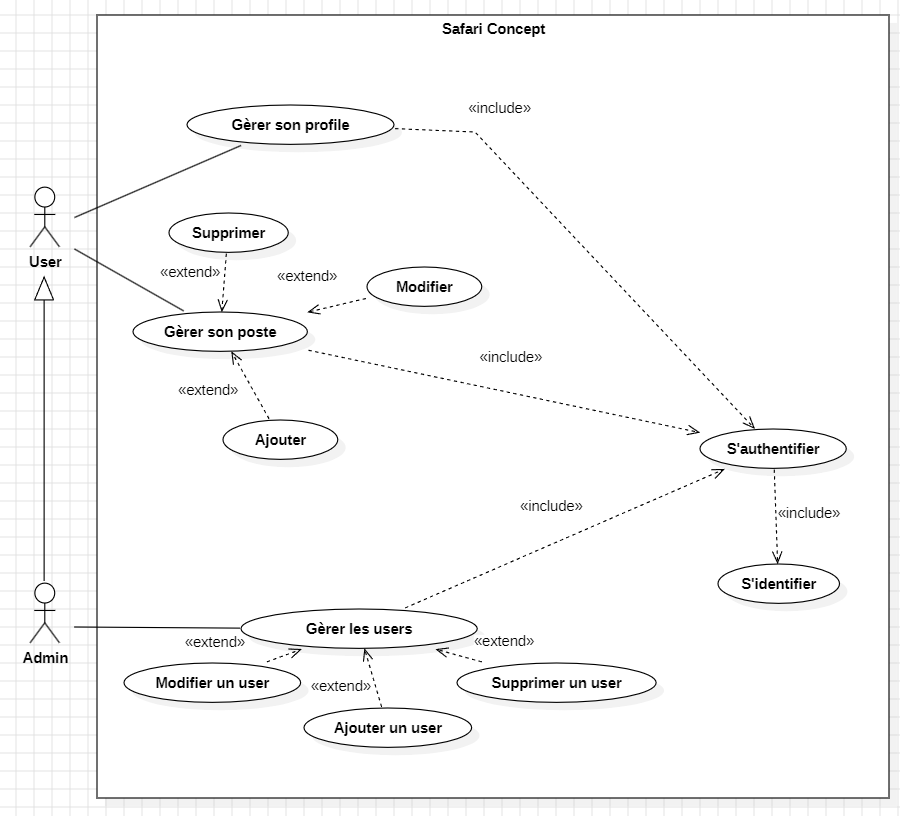
\includegraphics[width=0.9\textwidth]{images/image.png} 
    \caption{Diagramme de cas d'utilisation - "Safari"}
    \label{fig:Diagramme de cas d'utilisation - "Safari"}
\end{figure}

\paragraph{\\}

\section{Diagramme de Classe - "Safari"}

Le diagramme de classe est l’un des diagrammes les plus importants au 
niveau de la modélisation du logiciel/application, il montre non seulement 
la structure interne du système mais également une représentation 
abstraite des objets ( classes ) qui vont interagir entre eux.\\

Une classe est une description d’un groupe d’objet partageant un 
ensemble commun de propriétés, de comportements et de relations avec 
d’autres objets. Pour faire simple, il s’agit de :  Méthode ( autrement appelé opération ) - Attributs - Associations. \\

 \renewcommand{\thefigure}{2}
\begin{figure}[htbp]
    \centering
   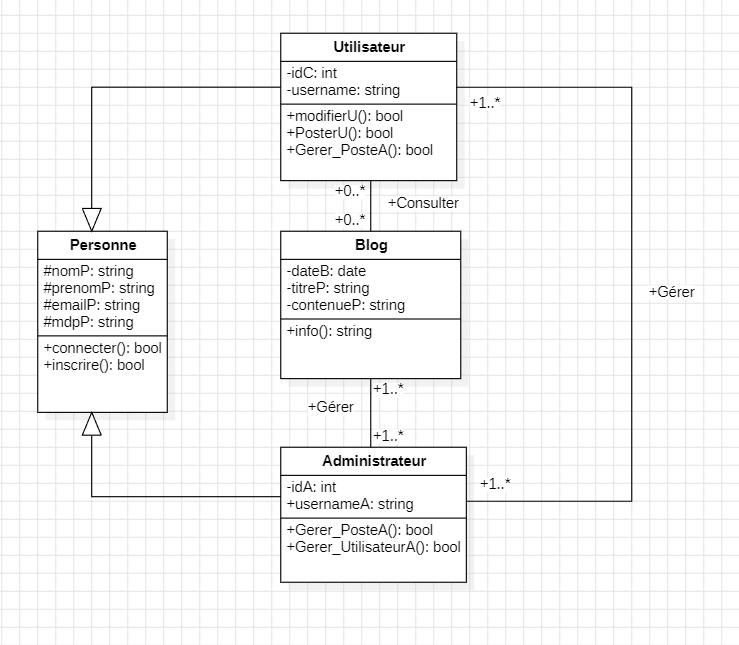
\includegraphics[width=0.8\textwidth]{images/image1.png} 
    \caption{Diagramme de Classe - "Safari"}

\subsubsection{Analyse et Lecture  :}

C’est pout cela, afin d’optimiser le diagramme on a décidé de mettre les 
points en commun dans une seule classe nommée Personne, ce dernier 
sera hérité par l'Utilisateur \& Administrateur. 
    \label{fig:Diagramme de classe - "Safari"}
\end{figure}

\end{enumerate}
 


\chapter{Réalisation - "Django"  }%
\label{chap5:introduction}
%% @Author: Ines Abdeljaoued Tej
%  @Date:   2018-06
%% @Class:  Graduation Project, ESSAI - Carthage University, Tunisia.

\section{Outil de Développement}

\begin{enumerate}
     \item \textbf{HyperText Markup Language}
    
 HTML permet la création de pages web basique. Il permet de mettre dans la zone la  Forme et le contenu d’une page web en utilisant une syntaxe composée.
\paragraph{\\}
 \renewcommand{\thefigure}{3}
    
    \begin{center}
        \begin{figure}[htbp]
    \centering
   \includegraphics[width=0.15\linewidth]{images/html (2).png} 
    \caption{Logo d'HTML}
   \paragraph{\\}\paragraph{\\}
    \label{fig:HyperText Markup Language}
\end{figure}
       
    \end{center}
    \paragraph{\\}

    \item \textbf{Framework Django}
    
 Django est une Plateform de développement web open-source en Python. Il fournit une structure ou architecture et des outils puissants pour la création rapide d'applications web    complexes et 100\% sécurisées.
     \renewcommand{\thefigure}{4}
    \begin{center}
        \begin{figure}[htbp]
    \centering
   
\includegraphics[width=0.3\linewidth]{images/django1.png} 
    \caption{Logo de Django}
    \label{fig:Framework Django}
\end{figure}
        
    \end{center}

        
          \paragraph{\\}\paragraph{\\}\paragraph{\\}
     \item \textbf{Cascading Style Sheets}
     
 CSS est un langage de feuilles de style utilisé pour la présenter visuellement des documents HTML. Il permet un contrôle total de  l'apparence des éléments d'une page web, tels que la couleur, la police, la taille du texte, la mise en page, etc.

 \renewcommand{\thefigure}{5}
    
    \begin{center}
        \begin{figure}[htbp]
    \centering
   \includegraphics[width=0.1\linewidth]{images/cdd1.png} 
    \caption{Logo de Css}
    \label{fig:Cascading Style Sheets}
\end{figure}
        
    \end{center}
    \paragraph{\\}\paragraph{\\}\paragraph{\\}

      
     \item \textbf{Python}
    
Le langage Python est un langage de programmation polyvalent et puissant utilisé pour développer des logiciels système, des logiciels de bureau, des jeux vidéo et bien plus encore. Python fournit un contrôle précis sur la manipulation de la mémoire et permet la création de programmes performants et efficaces.

 \renewcommand{\thefigure}{6}
    
    \begin{center}
        \begin{figure}[htbp]
    \centering
   \includegraphics[width=0.1\linewidth]{images/python1.png} 
    \caption{Logo de Python}
    \label{fig:Python}
\end{figure}
        
    \end{center}
   
   \paragraph{\\}
   
   \paragraph{\\}
  
    \paragraph{\\}\paragraph{\\}
  
 \section{Premier pas vers l'UI de - "Safari"}

À partir de cette première interface utilisateur, L’utilisateur disposera de deux choix : se connecter ou s’inscrire. Il suffit donc d’entrer son nom d'utilisateur et son mot de passe pour avoir accès au menu autrement appèles accueil.

\renewcommand{\thefigure}{7}

\begin{center}
    \begin{figure}[htbp]
        \centering
        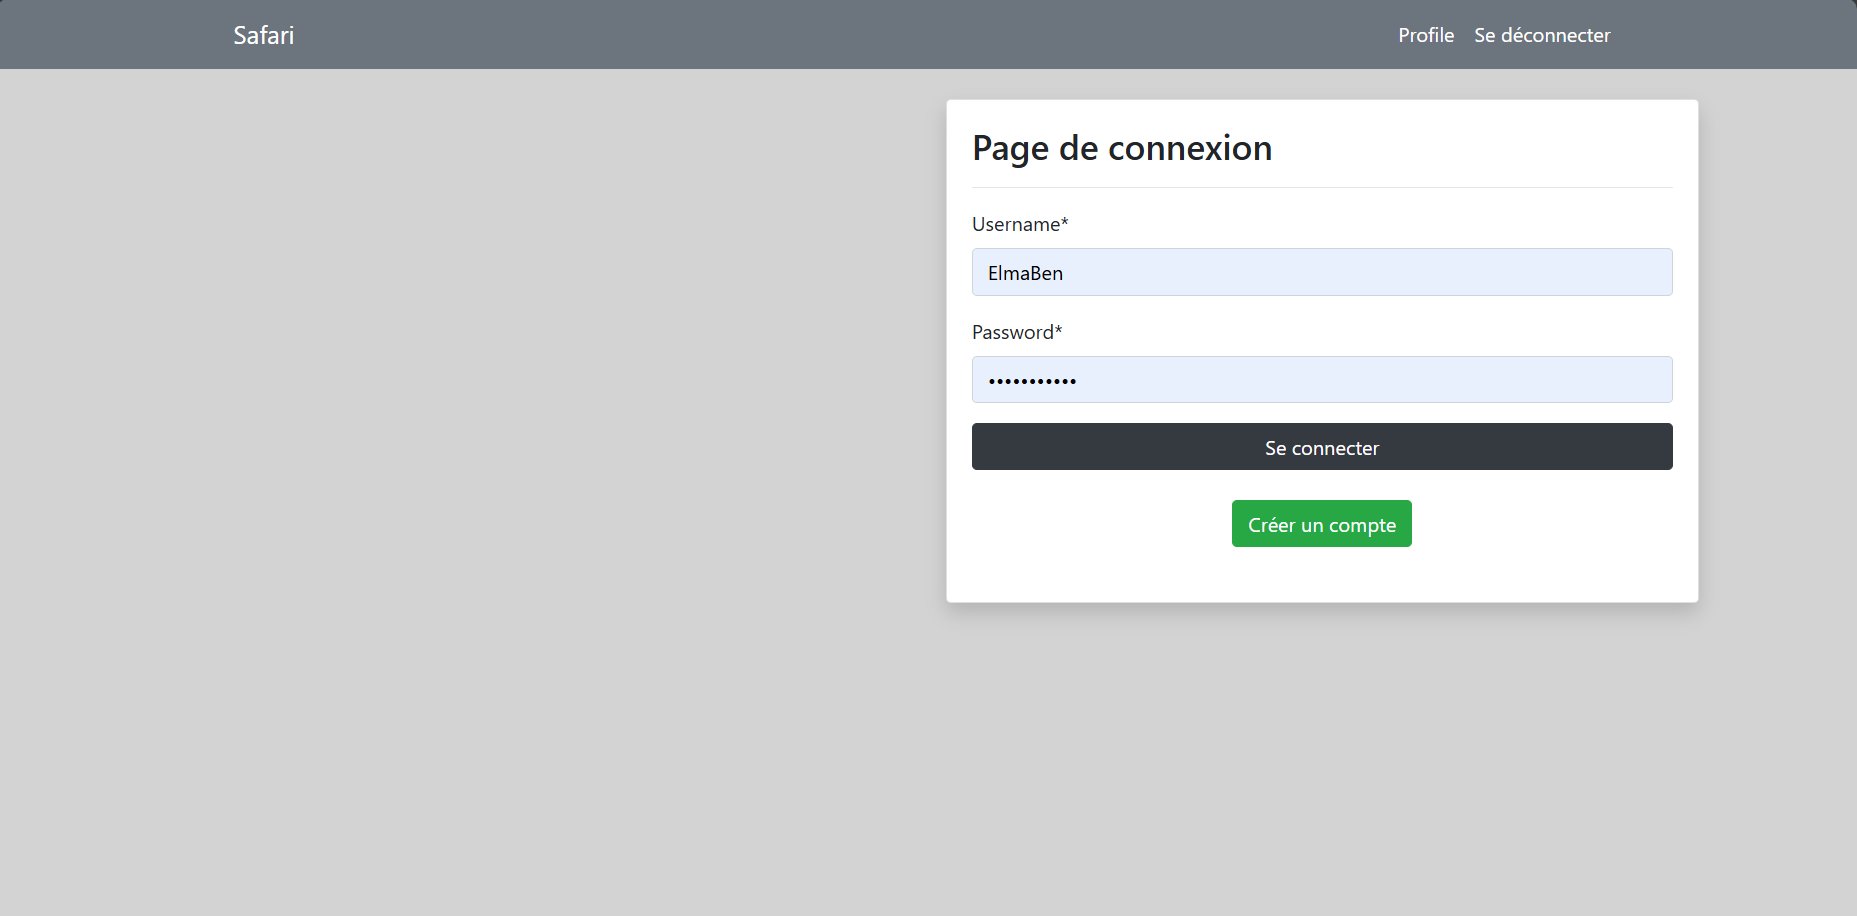
\includegraphics[width=\textwidth, height=0.8\textheight]{images/connexion_first.png} 
        \caption{Page de connexion}
        \label{fig:C++}
    \end{figure}
\end{center}

  \paragraph{\\}
  
    \paragraph{\\}
    \paragraph{\\}
  
  \paragraph{\\}
  \paragraph{\\}
  
    \paragraph{\\}
  
\section{Page D’inscription}

\renewcommand{\thefigure}{8}
  \paragraph{\\}
\begin{center}
    \begin{figure}[htbp]
        \centering
        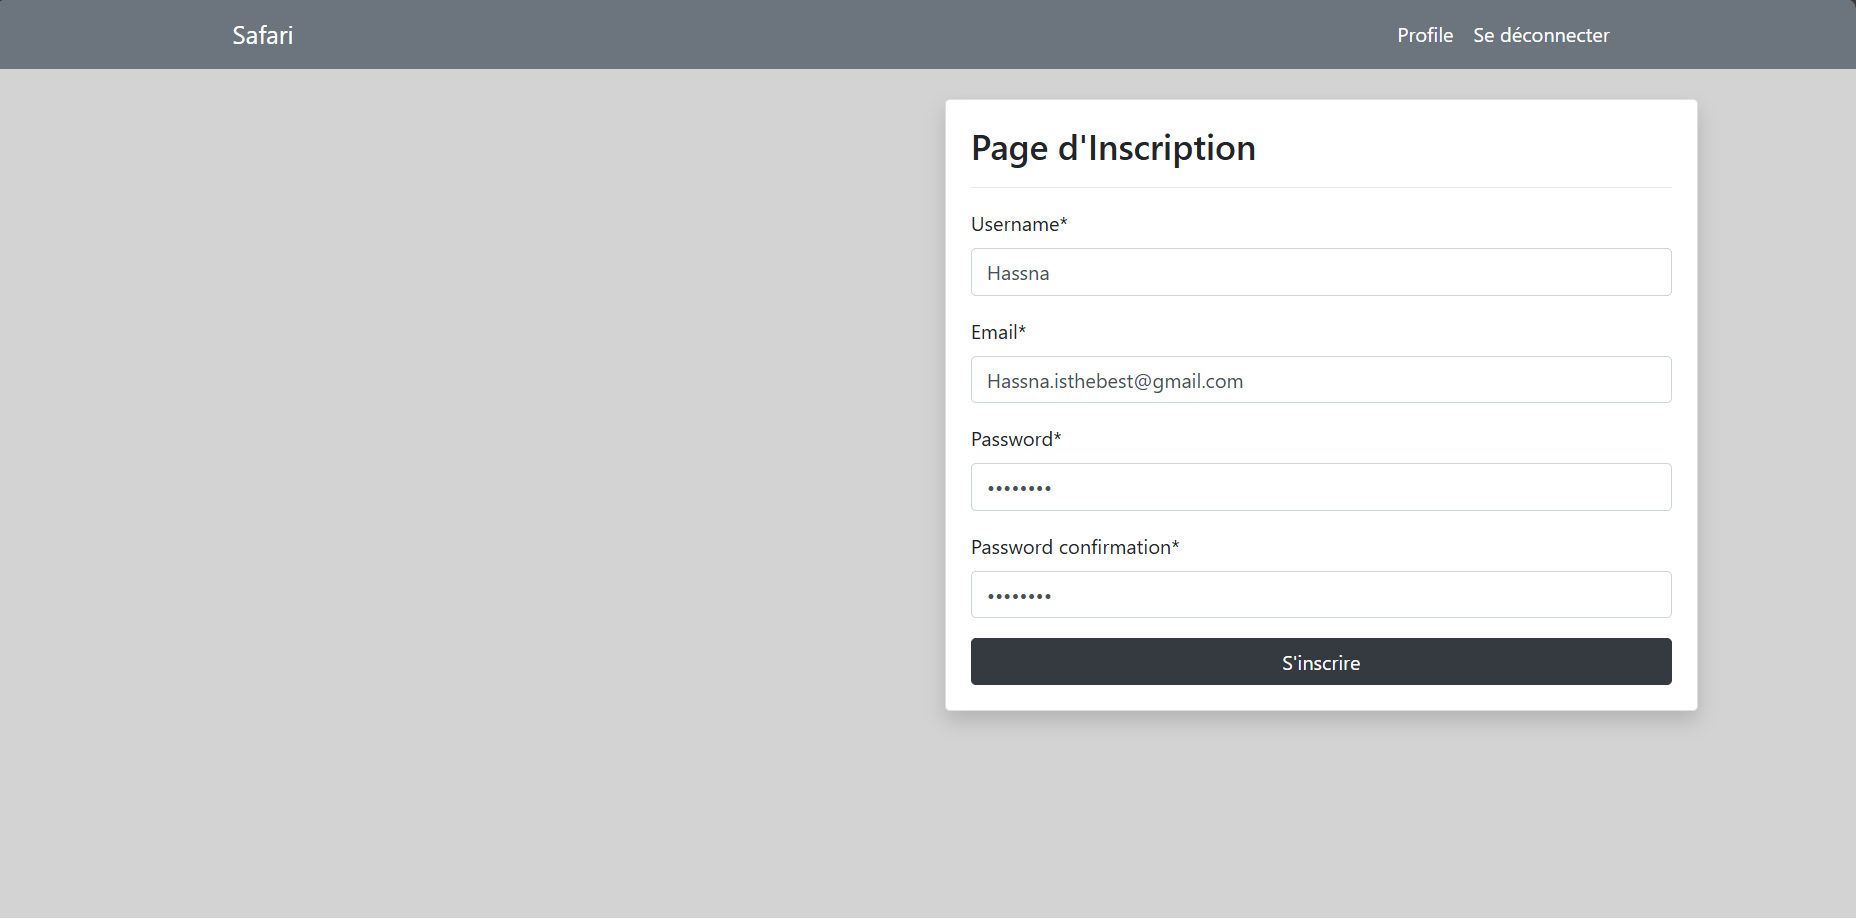
\includegraphics[width=1\linewidth, height=0.65\textheight]{images/inscription_second.png} 
        \caption{Page d'inscription}
        \label{fig:Page d'inscription}
    \end{figure}
\end{center}
 
  
  
  \paragraph{\\}
  
    \paragraph{\\}
  
\section{Page de Publication de Blog}

\renewcommand{\thefigure}{9}
  \paragraph{\\}
\begin{center}
    \begin{figure}[htbp]
        \centering
        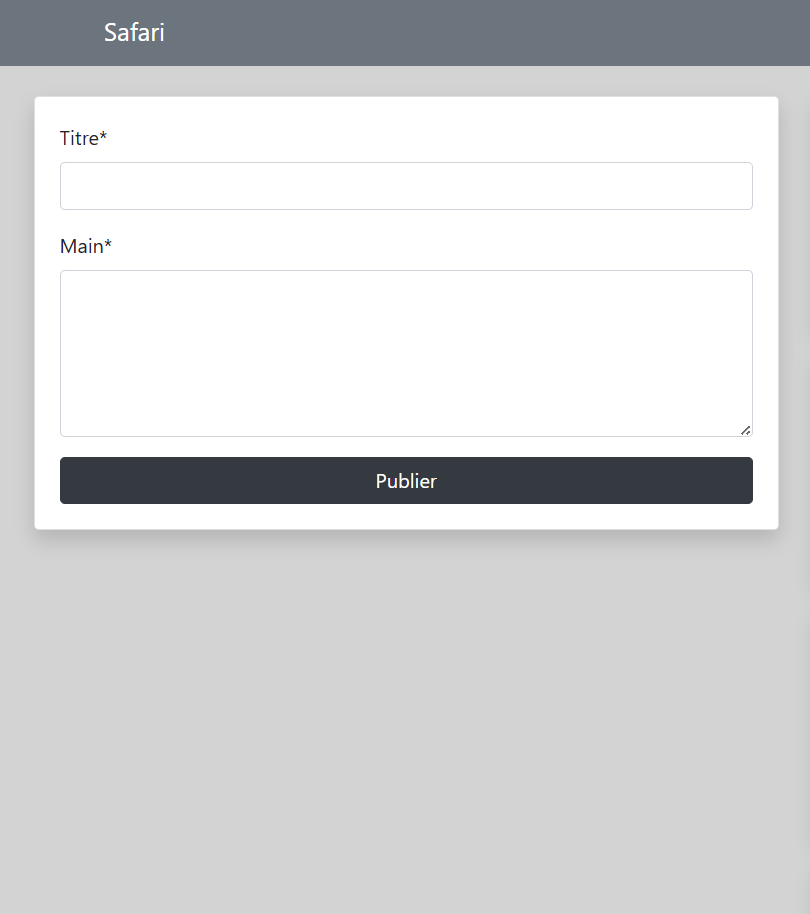
\includegraphics[width=1\linewidth, height=0.65\textheight]{images/publication_third.png} 
        \caption{Page de Publication de Blog}
        \label{fig:Page de Publication de Blog}
    \end{figure}
\end{center}
    
   
  \paragraph{\\}
  
    \paragraph{\\}
  
\section{Interface Admin}

\renewcommand{\thefigure}{10}
  \paragraph{\\}
\begin{center}
    \begin{figure}[htbp]
        \centering
        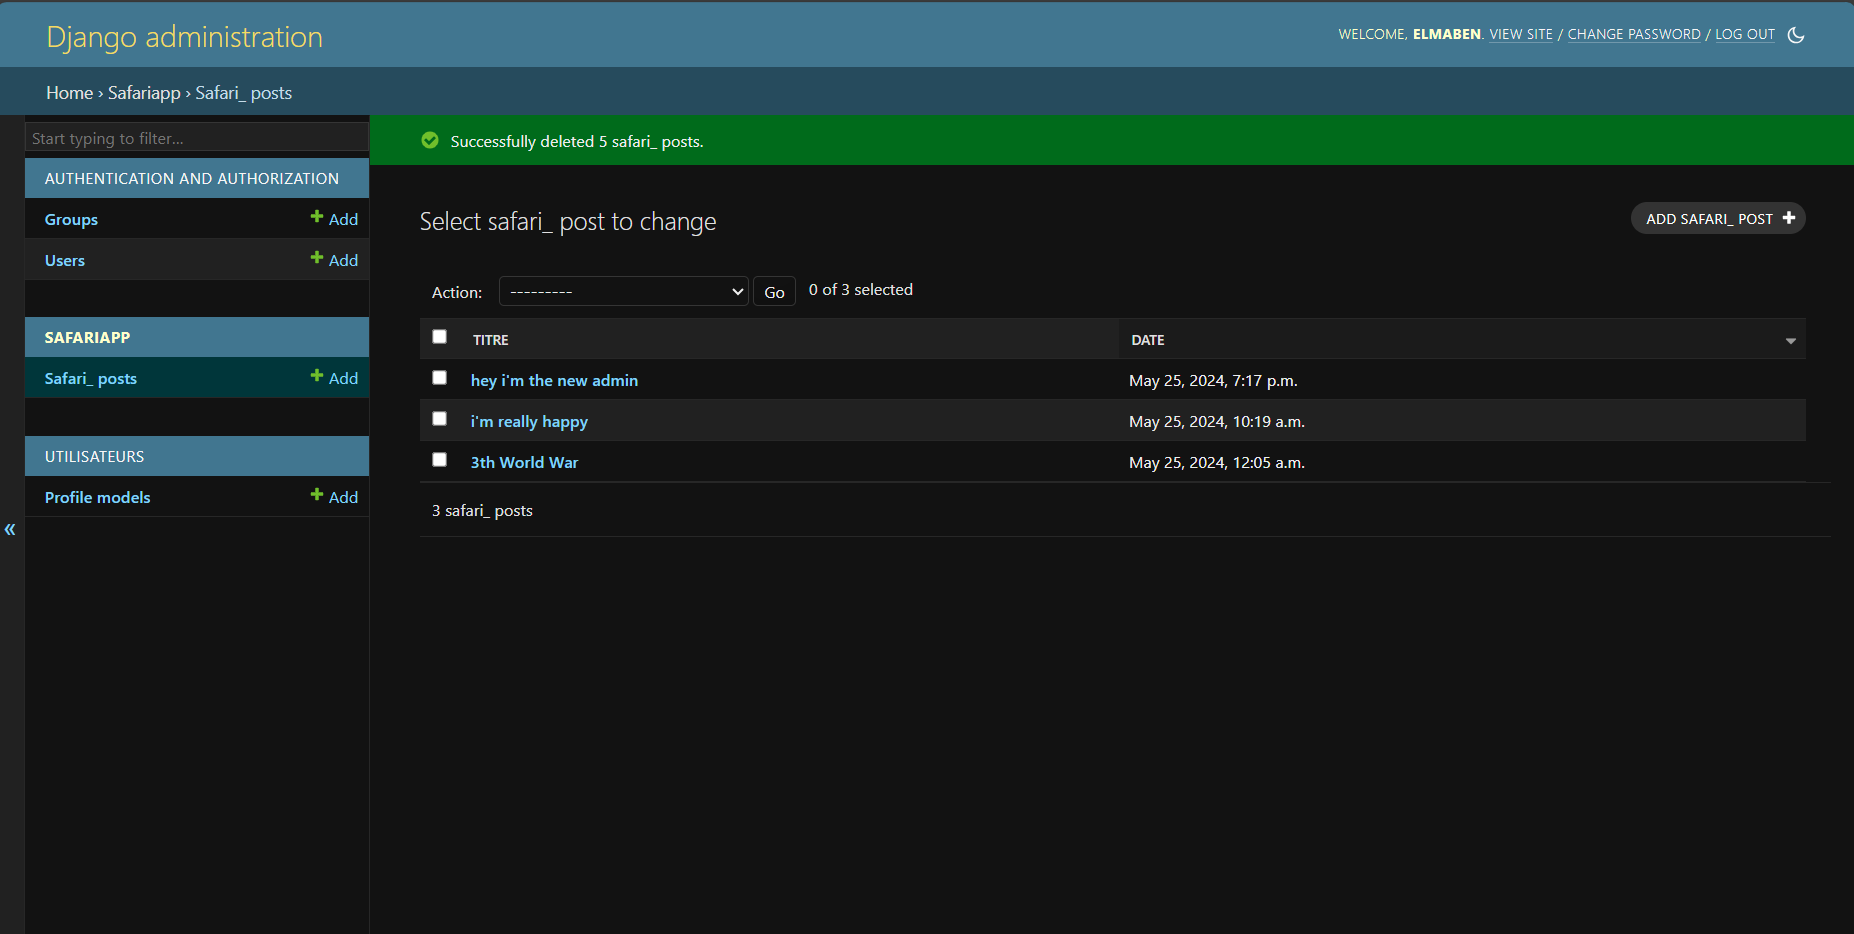
\includegraphics[width=1\linewidth, height=0.65\textheight]{images/Admin_Fourth.png} 
        \caption{Interface Admin}
        \label{fig:Interface Admin}
    \end{figure}
\end{center}
  
\end{enumerate} 

\label{chap:conclusion}

\chapter*{Conclusion}
\addcontentsline{toc}{chapter}{Conclusion}
\label{chap:conclusion}
%% @Author: Ines Abdeljaoued Tej
%  @Date:   2018-06
%% @Class:  Graduation Project, ESSAI - Carthage University, Tunisia.

\vspace{1cm}\vspace{1cm}\vspace{1cm}\vspace{1cm}\vspace{1cm}
Au terme de ce rapport, nous pouvons conclure que l’objectif est de 
développer une application de planification de Blog nommé Dream 
"Safari".  \\
Pour la développer nous avons utilisé plusieurs technologies, nous 
citons :  StarUML - VisualStudio et j'en passe
Cette application reste une première version "BETA", car elle lui manque beaucoup d'autre options. \\
Le présent travail, effectué au sein de l’école marocaine de science et de 
l’ingénieur, s’inscrit sous le cadre du projet de fin de semestre. Tout au 
long de l’élaboration du projet, nous avons rencontré plusieurs difficultés 
tant au niveau conceptuel qu’au niveau de l’implémentation et du temps. \\
Tout de même, nous avons à moitié réussi à les surpasser pour 
présenter en fin de compte une application opérationnelle.  
Nous espérons que le travail que nous avons effectué a été à la hauteur 
de la confiance qui nous a été donnée. 

 
 


%%%%%%%%%%%%%%%%%%%%%%%%%%%%%%%%%%%%%%%%%%%%%%%%%%%%
% Don't touch this, it is auto generated
%%%%%%%%%%%%%%%%%%%%%%%%%%%%%%%%%%%%%%%%%%%%%%%%%%%%
\nocite{*}

%\phantomsection{}
%\addcontentsline{toc}{chapter}{Webography}
%\printbibliography[title={Webography},type=online]

%\phantomsection{}
%\addcontentsline{toc}{chapter}{Bibliography}
%\printbibliography[title={Bibliography},nottype=online]

%\printbibheading %exemple de bibliographie divisée en sections. Pour ajouter des oeuvres non citées,utiliser \nocite

%\printbibliography[keyword=pratique,heading=subbibliography,title={Théories littéraires dans les jeux vidéo}]
%\printbibliography[keyword=litteraire,heading=subbibliography,title={Narratologie et structuralisme}]

%\printbibliography[keyword=jeu,heading=subbibliography,title={\emph{Games studies}}]

\bibliographystyle{apalike}
%\bibliographystyle{plain}

\bibliography{Biblio.bib}


@book{robbins2018learning,
  title={Learning Web Design: A Beginner's Guide to HTML, CSS, JavaScript, and Web Graphics},
  author={Robbins, Jennifer Niederst},
  year={2018},
  publisher={O'Reilly Media}
}

@book{crockford2008javascript,
  title={JavaScript: The Good Parts},
  author={Crockford, Douglas},
  year={2008},
  publisher={O'Reilly Media}
}

@book{haverbeke2018eloquent,
  title={Eloquent JavaScript: A Modern Introduction to Programming},
  author={Haverbeke, Marijn},
  edition={3},
  year={2018},
  publisher={No Starch Press}
}

@book{vincent2018django,
  title={Django for Beginners: Build websites with Python and Django},
  author={Vincent, William S.},
  year={2018},
  publisher={Independently published}
}

@book{williams2017professional,
  title={Professional WordPress: Design and Development},
  author={Williams, Brad and Damstra, David and Stern, Hal},
  edition={3},
  year={2017},
  publisher={Wrox}
}

@book{krug2014dont,
  title={Don't Make Me Think: A Common Sense Approach to Web Usability},
  author={Krug, Steve},
  edition={3},
  year={2014},
  publisher={New Riders}
}






\cleardoublepage%

\addtocontents{toc}{\protect\setcounter{tocdepth}{3}}

\printglossaries
\printindex

%
% les tests de performance 
\keywords{}
\keywordss{} \\

\vspace{3cm}
\centerline{\bf Abstract/Résumé}
\vspace{0.6cm}


\keywords{}
\keywordss{}




\end{document}
